\begin{withoutheadline}
\begin{frame}
\vspace*{-13mm}
\begin{figure}
	\hspace*{-4.2mm}
    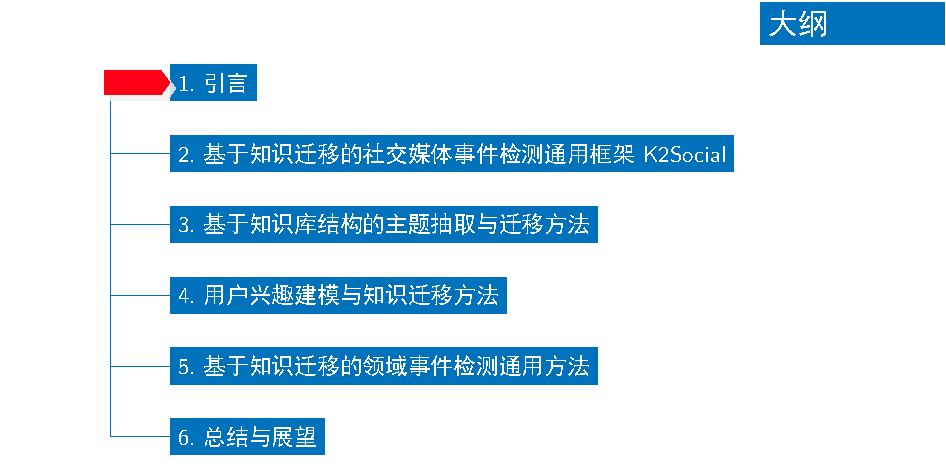
\includegraphics[width=1.0\paperwidth]{img/contents1_output.pdf}
\end{figure}
\end{frame}
\end{withoutheadline}

\section{引言}
%------------------------------
\begin{frame}
\frametitle{社交媒体事件检测问题的背景}

\begin{figure}
    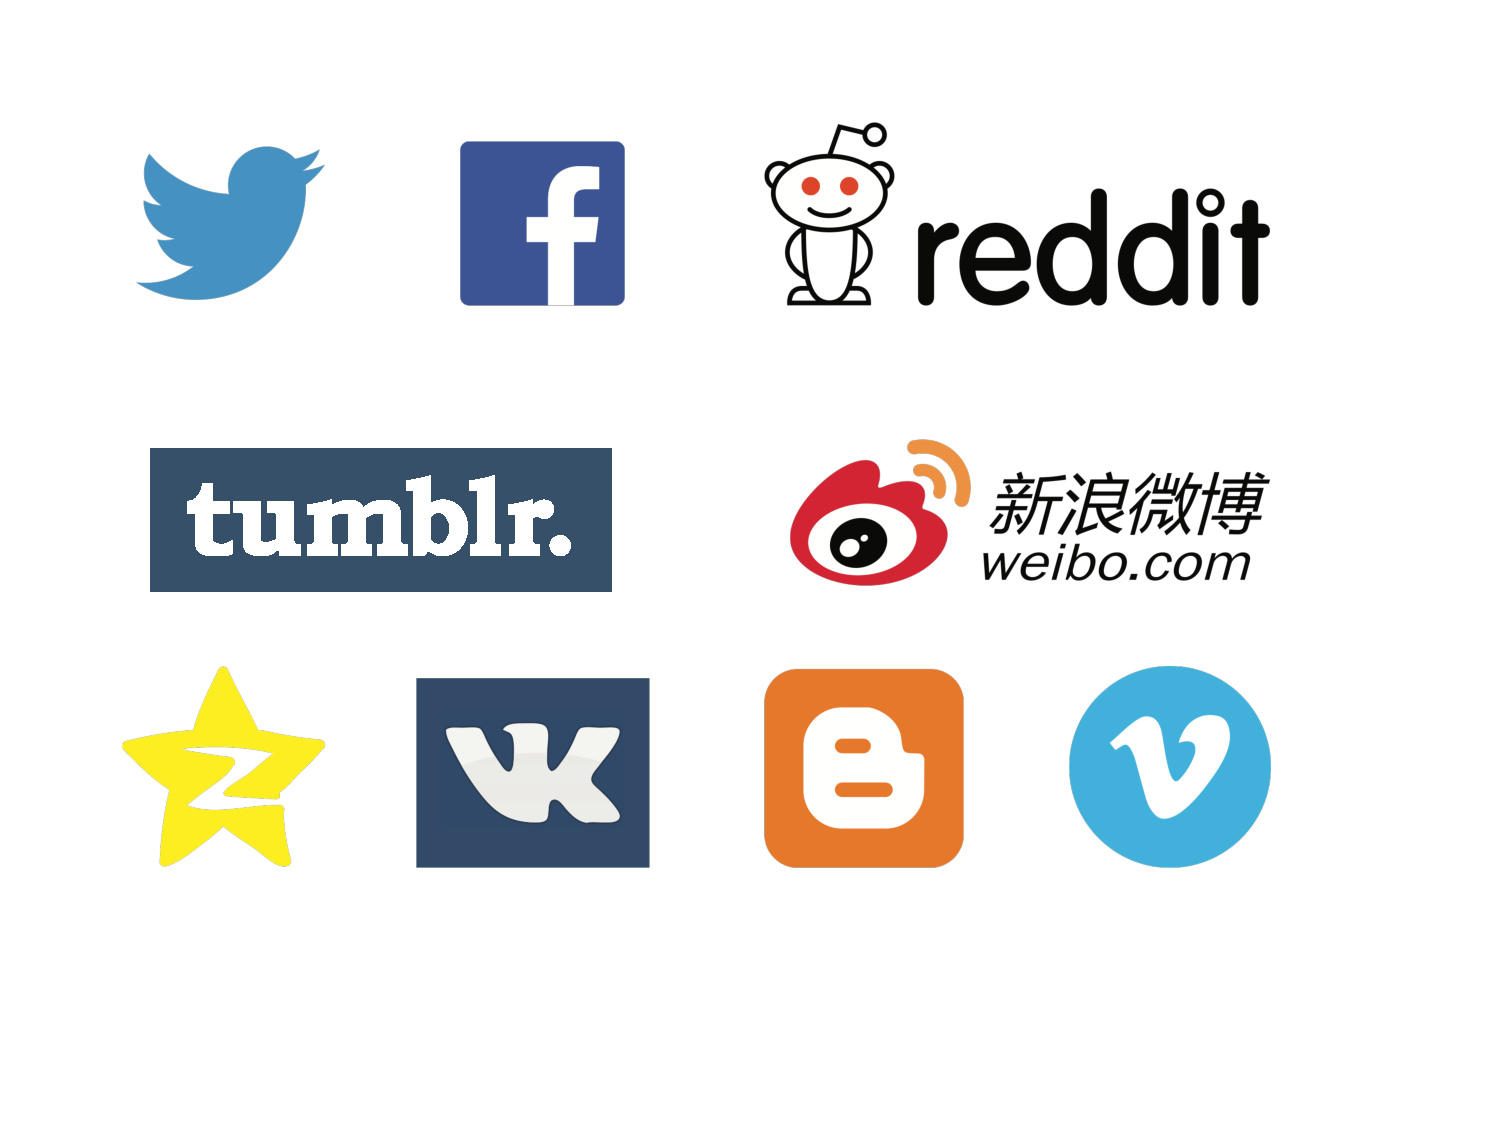
\includegraphics[width=0.75\paperwidth]{img/logos.pdf}
\end{figure}

\end{frame}


%------------------------------
\begin{frame}
\frametitle{社交媒体事件检测问题的背景}
社交媒体上进行事件检测可服务于众多应用:
\begin{figure}
    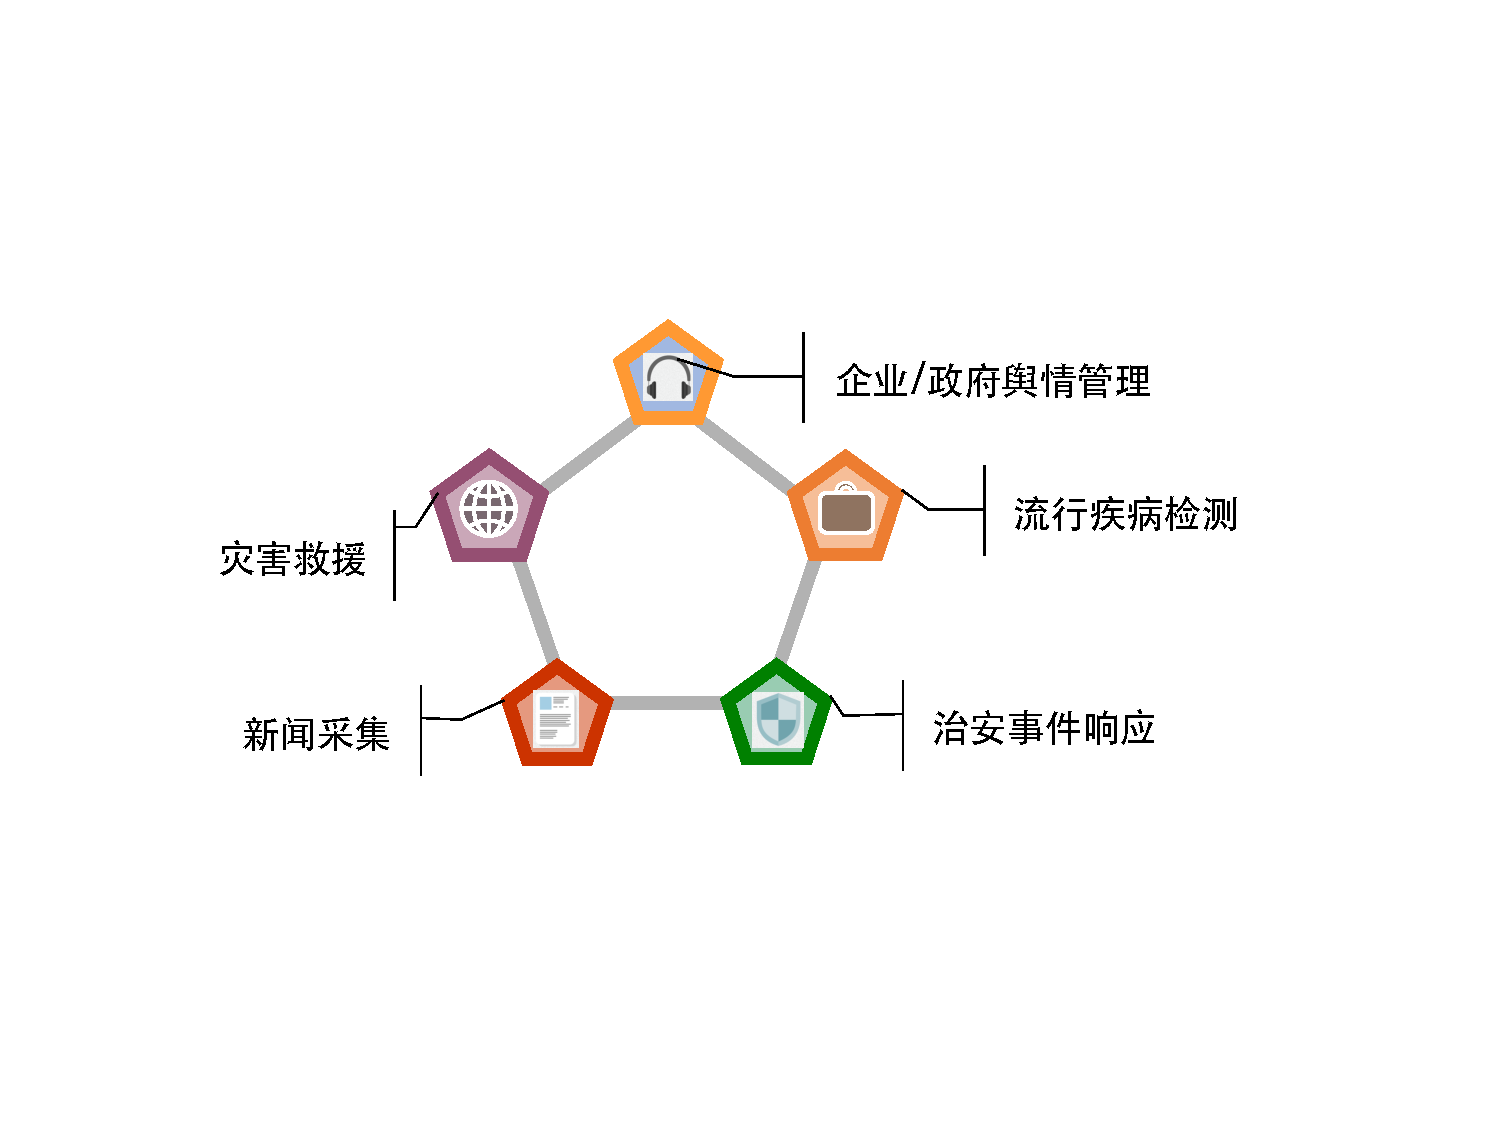
\includegraphics[width=0.75\paperwidth]{img/event_applications.pdf}
\end{figure}

\end{frame}

%------------------------------
\begin{frame}
\frametitle{社交媒体的语境动态演变及带来的挑战}
\onslide<1-4>{
\begin{tcolorbox}[colback=red!5,colframe=red!75!black]
社交媒体用语不规范,主题动态变化,我们将其总结为社交媒体的语境动态演变
\end{tcolorbox}
}

\vspace{-5mm}

\begin{columns}[onlytextwidth, t]
\column{0.32\linewidth}
	\onslide<2-4>{
    \begin{tcolorbox}[colback=red!5,colframe=red!5]
    交流语境的变化:从正式交流语境到非正式交流语境的转变,导致用语不规范[Gunraj 2016].
    \end{tcolorbox}
    }

\column{0.32\linewidth}
	\onslide<3-4>{
    \begin{tcolorbox}[colback=red!5,colframe=red!5]
    外部语境的变化:用户易于被外界影响[Weng 2012],热门话题随着时间快速变化。
    \end{tcolorbox}
    }
    
\column{0.32\linewidth}
	\onslide<4>{
    \begin{tcolorbox}[colback=red!5,colframe=red!5]
    前述两种变化的综合叠加,例子:Somehow made it through Irene. 仅在2011.8的语境中知道这是关于飓风艾琳。 
    \end{tcolorbox}
    }
\end{columns}

%\begin{tcolorbox}[colback=red!5,colframe=red!75!black]
%外在表现:用语不规范,主题动态变化
%\end{tcolorbox}


\end{frame}


%------------------------------
\begin{frame}
\frametitle{社交媒体的语境动态演变及带来的挑战}

\begin{table}[]
\centering
\caption{社交媒体事件检测已有方法}
\scalebox{0.75}{
\begin{tabular}{|c|c|c|c|c}
\cline{1-4}
方法类型 & 代表工作 & 事件粒度 & 特点 &  \\ \cline{1-4}
基于普通聚类的方法 & {[}Chen, SIGIR 2013{]} & 高频的相似微博 & 实现简单 &  \\ \cline{1-4}
基于敏感哈希的方法 & {[}Petrovic, NAACL 2010{]} & 高频的相似微博 & 响应速度快 &  \\ \cline{1-4}
基于词频统计的方法 & {[}HE,SIGIR 2007{]} & 高频词组 & \begin{tabular}[c]{@{}l@{}}可区分周期性、\\ 非周期性事件\end{tabular} &  \\ \cline{1-4}
基于主题模型的方法 & {[}Yan, AAAI 2015{]} & 主题 & 可利用上下文信息 &  \\ \cline{1-4}
基于分类器+后处理 & {[}Yang, KDD 2014{]} & \begin{tabular}[c]{@{}l@{}}对微博分类后,\\ 再检测事件\end{tabular} & 进行领域事件检测 &  \\ \cline{1-4}
\end{tabular}
}
\end{table}

{\color{blue} 受限于社交媒体的语境动态演变,上述方法难于准确检测事件。}
\end{frame}